\chapter{Developer Documentation} % Developer guide
\label{ch:impl}

In this chapter, we are going to dive deep into the details of creating the log analyzer,
the architecture, and why the different parts of it were necessary, and how they all fit together.

To build and run the project as a developer, it is the same steps as in \ref{sec:installiation_guide}.
The user is expected to be able to add to the analyzer to match their different need and that is why
the roles of the developer and the user are very close to each other in the project.

As mentioned before, the log analyzer and the profiler are very tight, and to understand the analyzer's
design and its components, an overview of the profiler is needed. The next section covers this overview.
\newline
\begin{figure}[H]
	\centering
	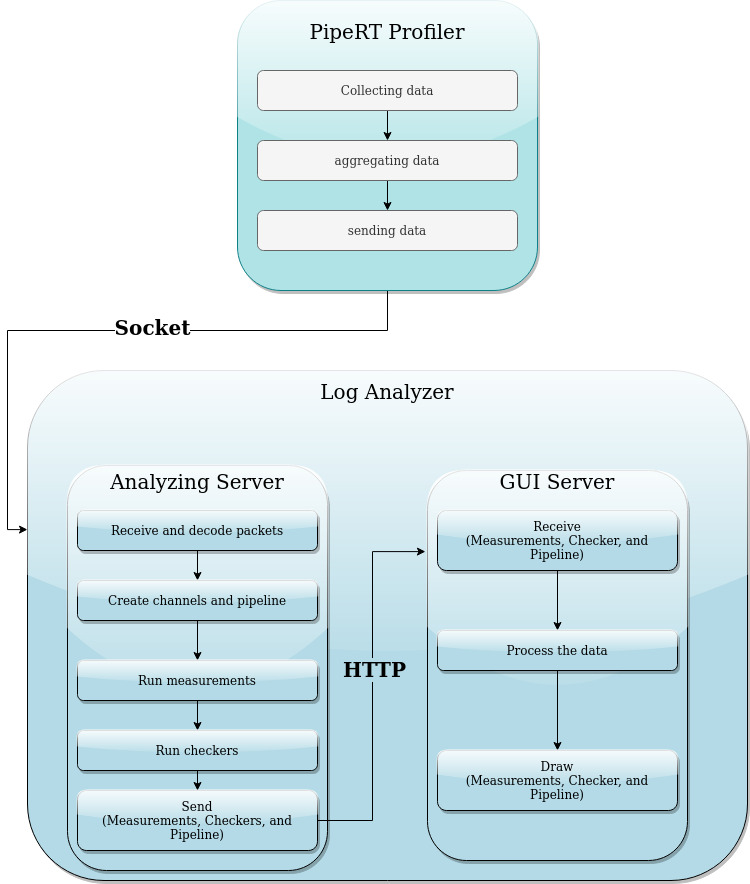
\includegraphics[width=0.9\textwidth,height=380px]{images/general_work_flow.jpg}
	\caption{General workflow}
	\label{fig:general_work_flow}
\end{figure}

\section{PipeRT Profiler}\label{sec:profiler}
The profiler is the utility in PipeRT responsible for profiling and monitoring functionality. It is a
sub-system to collect, aggregate, serialize, and send data to the log analyzer. The different configurations
of the profiler can be found at \ref{sec:server_side_config}.

The collection and aggregation of the profiler happen over different types of  events, there exist several
predefined events, however, the user can also add their events if needed. These different events are
the analyzer guideline for the channels' measurements and to understand the pipeline and measure it.

\subsection{Events}\label{sec:events}
The events are actions that happen to a packet in a channel. There are six predefined events, \textbf{Pushed},
\textbf{Retrieved}, \textbf{Execution Time}, \textbf{Fill Time}, \textbf{Read Time}, and \textbf{Dropped Packet}.

Since the profiler is supposed to aggregate these events, the \textit{log aggregator}, a helper utility in the profiler, is going to group these events
based on the event type, and these aggregated data will be sent to the log analyzer. Each aggregated event will have
a log count, and that is the number of logged events, and the time aggregation started, minimum,
maximum, and the average time that event took to complete.

\subsubsection{Pushed Event}\label{sec:pushed_event}
Time in packet's timeline when the packet is filled with data and pushed into the channel buffer.

\subsubsection{Retrieved Event}\label{sec:retrieved_event}
Time in packet's timeline when the packet is retrieved for processing.

\subsubsection{Execution Time Event}
Time spent by a scheduler thread servicing a channel callback.

\subsubsection{Fill Time Event}
Time spent between acquiring the packet and pushing it into the buffer

\subsubsection{Read Time Event}\label{sec:read_time_event}
Time spent between retrieving a packet and releasing it by the retriever

\subsubsection{Dropped Packet Event}
Packet was dropped because the buffer of a channel was full when the packet arrived.

\subsection{Sending Data} \label{sec:sending_data}
The profiler has a \textit{Sender Logger} auxiliary utility, which is responsible for serializing and sending
the data aggregated by the profiler. The sending part is the bridge of communication between the Profiler
and the analyzer so it was very important to consider the different possibilities before choosing the appropriate one.

Sending through sockets was the choice in sending and it is normal to use with such application, but the serialization
was not as clear of a choice, there are various ways to serialize the data, we are going to discuss four of them,
\textbf{binary sending}, \textbf{strings}, \textbf{XML} (Extensible Markup Language), and \textbf{protobuf} \cite{protobuf}.
Each one of them has its pros and cons.

Turn the data into a string is costing building the string and also any changes will mean changes in the
receiving side as well. The useful outtake of this option is the straightforward implementation.

Using XML as a format to communicate is a big burden on the performance and can lead to high memory usage,
that said XML is a very popular format and a go-to option based on the project.

Protobuf or protocol buffers from \textit{Google} is a work out of the box experience but will cost
extra maintenance in the long run and can be slow.

The final decision was using \textbf{binary sending}, despite that choosing this will lead to always make
sure that the profiler and analyzer are up to date with each other's sending and receiving
changes, the performance will be better compared to the other possibilities, and this performance
difference is an important key to minimize the delay hence having a better live analyzing which is the
main goal for the log analyzer.

\subsection{Packet serialization}\label{sec:packet_serialization}
The profiler sends packets of bytes, all the packets have the same structure, starts with \textit{DGRP}
as declaration of a new packet, null-terminated string of the receiver channel, 
\textit{SEND}, a null-terminated string of the sender channel, arbitrary number of aggregated data starts
with \textit{LOGA}, a null-terminated string of event's type, four bytes integer for \textit{log count}, 
four bytes integer for \textit{time passed in microseconds}, eight bytes double for \textit{minimum value}, 
eight bytes double for \textit{maximum value}, and eight bytes double for \textit{average value}.
\newline
\begin{figure}[H]
	\centering
	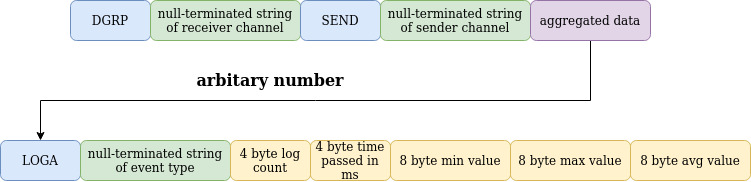
\includegraphics[width=1.0\textwidth,height=200px]{images/packet.jpg}
	\caption{Packet's structure}
	\label{fig:packet_structure}
\end{figure}

sending the packets is the last step in the profiler's workflow (\ref{fig:general_work_flow}) 
and from there, the log analyzer will start receiving and analyzing.

The log analyzer is separated into two main parts, as can be seen from \ref{fig:general_work_flow}.
In the next sections, details about these parts, their different components, and the connection between
them will be our topic.

\section{The Analyzing Server}
The first and the most vital part of the two, its importance comes from its responsibility
to hold the logic of the analyzing, reading configuration, sending the data to the \textbf{GUI server}.
The coding of the \textbf{analyzing server} was done in \textit{Python3} and the language choice was because
it is easy to use and fast to develop in which is suitable since it is expected from the user of the
analyzer to extend it.


The \textit{Front Controller Pattern} is the most used in the design of the \textbf{analyzing server},
and it is used to provide a centralized request handling 
mechanism so that all requests will be handled by a single handler which is very suitable to the various
checkers and measurements in the project.

\textbf{AnalyzerServer} is the heart class of the \textbf{analyzing server} so it is the main controller
and responsible of starting and providing data for other controllers.

The first task for the \textbf{analyzing server} is to receive the packets from the profiler and decode it.

\subsection{Receiving and Decoding Packets}
Configuring the ip and port is crucial for successful receiving, the \textit{socket} library in \textit{Python}
is used to create the server and listen to the upcoming requests. The implementation of the server is
inside the \textbf{AnalyzerServer} class and upon receiving the packets the class is starting running the
other controllers.

The \textbf{PacketsManager} is the controller responsible for decoding the packets and distinguish them
by giving each of them different id number, it has two main methods, \textbf{add} to decode and add new packet
and \textbf{get\_latest\_packet} which is used as an input for the \textbf{ChannelsManager}. The \textit{sigleton} 
desgin pattern was used to implement the \textbf{PacketsManager} as to have single instance of it 
everywhere in the code.
\newline
\begin{lstlisting}[language=Python, label=PacketsManager, caption={Puplic methods of PacketsManager},captionpos=b]
def add(self, packet):
	packet = PacketDecoder(packet).decode_packet()
	packet.set_id(self.__packets_count)
	packet.set_id_for_events()
	self.__latest_packet = packet
	self.__packets_count += 1

def get_latest_packet(self):
	return self.__latest_packet

def get_packet_count(self):
	return self.__packets_count

\end{lstlisting}

The packet is represented as \textbf{Packet} class, and it contains all the information that is sent
in the packet from the profiler (\ref{sec:packet_serialization}), and also has an id which is set by the
\textbf{PacketsManager}. The packet object has a method to set id for the events in it, and this method
is used by its controller as can be seen in \ref{PacketsManager}.

The event is also represented as \textbf{Event} class and contains the data for the type, log count, 
passed time, minimum value, maximum value, and average value. The packet can have more than one event
as mentioned in \ref{sec:events}, and that is represented as a list of events objects in the packet object.

The \textbf{PacketDecoder} is the utility responsible for decoding and insinuating the packet object. But
before going into details about how the decoding takes place, \textit{endianness} should be discussed first.

\textit{Endianness} is the order or sequence of bytes in computer memory. 
it is primarily expressed as big-endian (BE) or little-endian (LE). 
A big-endian system stores the most significant byte at the smallest memory address and 
the least significant byte at the largest. A little-endian system, in contrast, stores 
the least significant byte at the smallest address.
\newline
\begin{figure}[H]
	\centering
	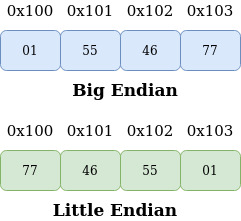
\includegraphics[width=0.9\textwidth,height=150px]{images/endianess.jpg}
	\caption{BE vs LE}
	\label{fig:be_vs_le}
\end{figure}
Since the packets comes in bytes (\ref{sec:sending_data}), the endianess of the bytes can form
an obstacle while decoding, \textit{Python} has built-in utilities to overcome that and these utilities
were used in the decoding such as \textbf{decode} method for strings, \textbf{from\_bytes} method for integers,
and \textbf{unpack} method in \textbf{struct} data structure for double values.
\newline
\begin{lstlisting}[language=Python, label=code:decoding, caption={Decoding of a packet},captionpos=b]
def decode_packet(self):
	pos = 0
	if self.__check_for_correct_packet(self.__packet[pos:pos+4]):
		pos += 4
		receiver_channel_name, pos = self.__get_keyword(pos)
		sender_channel_name, pos = self.__get_keyword(pos)
		events = []
		correct_packet = self.__check_for_correct_packet(self.__packet[pos:pos+4])
		while not correct_packet and pos < len(self.__packet):
			event, pos = self.__get_event(pos)
			events.append(event)
		return Packet(receiver_channel_name, sender_channel_name, events)
	else:
		raise ValueError
\end{lstlisting}
Code \ref{code:decoding} is showing the \textbf{decode\_packet} method in the \textbf{PacketDecoder}
class, the algorithm is straightforward as it is following the bytes order from figure \ref{fig:packet_structure}.
\newline
\begin{lstlisting}[language=Python, label=code:decoding_methods, caption={Helper methods in decoding},captionpos=b]
def __get_keyword(self, pos):
	keyword = b""
	while self.__packet[pos] != b"\x00":
		keyword += self.__packet[pos]
		pos += 1
	return keyword.decode("utf-8"), pos+1

def __get_int_val(self, pos):
	ret = b""
	for i in range(0, 4):
		ret += self.__packet[pos + i]
	pos += 4
	ret = int.from_bytes(ret, byteorder="big")
	return ret, pos

def __get_float_val(self, pos):
	ret = b""
	for i in range(0, 8):
		if byteorder == "little":
			ret += self.__packet[pos+(7-i)]
		else:
			ret += self.__packet[pos+i]
	[ret] = struct.unpack('d', ret)
	pos += 8
	return ret, pos
\end{lstlisting}

Code \ref{code:decoding_methods} shows the usage of the \textit{Python} decoding utilities mentioned before
and how they can be used for different types.

The next step after decoding is managing the channels and assign the events to the correct channels.

\subsection{Channels}
Every measurement and checker depends on channels, so that makes them the part holding much information
about the pipeline and the system performance. Each channel is represented by the \textbf{Channel} class,
and the controller for these channels is the \textbf{ChannelsManager} class.

The \textbf{Channel} class is responsible for representing the channel so it contains basic fields 
for name and events. The class is also storing the different checkers' flags and measurements. Each channel
is only storing events during the packet cycle as mentioned in \ref{sec:g_config}, the last packet id that
has been added to the channel is also stored as it is needed for measurements.

The \textbf{Channel} class is not only storing the measurements but also responsible for providing them
to send them to the \textbf{GUI server}, and different approaches were used to find a suitable logic.

\subsubsection{Checkers approach}
Checkers are sent at the end of every packet cycle, and as a first approach the measurements were sent
in the same way, but this leads to two issues, firstly, the \textbf{GUI server} has to update and redraw
the graphs too frequently that in a case when the profiler is sending very frequently the browser might
stop, secondly, not every measurement is worth of plotting, for example when having ten packet cycles with
the same measurement.

\subsubsection{Buffering approach}
We encountered two obstacles in this approach, the intention was to slow down the sending of the measurements
so that the browser can draw the graphs without overloading it. Instead of sending in every packet cycle,
the measurements are going to be stored in lists, and once the \textbf{AnalyzerServer} is requesting the measurements
the channel is going to send them, and empty the lists and this repeat every specific number of cycles. It is
implemented to be ten cycles for now.

\subsubsection{Buffering and RDB approach}\label{sec:buffering_rdb}
The buffering approach was successfully able to deal with the first obstacle, but that leaves the problem of
having unnecessary points in the graphs, to solve this issue, the \textit{Ramer–Douglas–Peucker algorithm} was introduced
in the implementation to reduce the number of plotted points. The \textit{Ramer–Douglas–Peucker algorithm}
also known as the \textbf{Douglas–Peucker algorithm} and \textbf{iterative end-point fit algorithm}, 
is an algorithm that perserve the shape of the curve with fewer points on it. 
It was one of the first successful algorithms developed for cartographic generalization. \cite{rdp}

The \textbf{Ramer–Douglas–Peucker algorithm} has it is own optimized library in \textit{Python} \cite{rdp_library},
and it was used to reduce the number of measurements in the graphs.
\newline
\begin{lstlisting}[language=Python, label=code:rdp, caption={Using rdp to reduce points},captionpos=b]
def reduce_points_n_extract_x_axis(points):
    minimized_points = rdp(points, epsilon=0.5)
    ret_points = [None] * 10
    for point in minimized_points:
        index = int((point[0] % 10) - 1)
        ret_points[index] = point[1]

    return ret_points
\end{lstlisting}

The \textbf{Ramer–Douglas–Peucker algorithm} calculations to reduce the points are based on epsilon's value,
and based on the choice of it, results can differ from each other on a small scale, but for the analyzer using
\textbf{0.5} is general enough for the use case so it was implemented as can be seen from \ref{code:rdp}.
\newline
\begin{figure}[H]
	\centering
	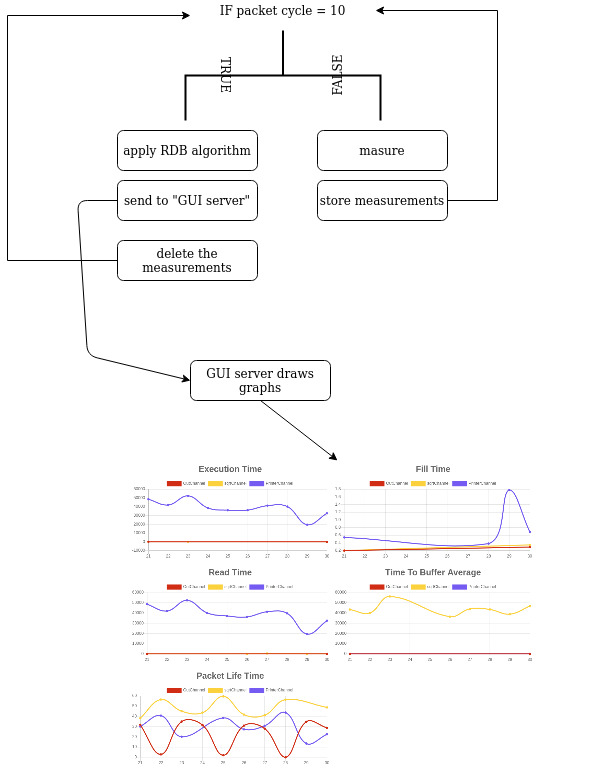
\includegraphics[width=1.0\textwidth,height=410px]{images/measurement_sending_cycle.jpg}
	\caption{Measurements sending mechanism}
	\label{fig:measurement cycle}
\end{figure}

The \textbf{ChannelsManager} is responsible for adding new channels, adding events for existent channels,
and creating the channels' map. It also contains a list of the channels in the pipeline 
and has a getter method to provide this list for the measurements or the checkers. Similar to the 
\textbf{PacketsManager}, the \textbf{ChannelsManager} is also implemented using a singleton design pattern.

In some packets, the sender is N/A channel which means that the channel has been fed data from a different
source other than the channels, for example, the first channel in the pipeline.

The \textbf{add\_packet} public method of it is used in the \textbf{AnalyzerServer}
and it is adding the receiver and the sender channels of the given packet. Adding the receiver is 
a matter of searching for the new channel name if it is not in the list, create a new channel
and add the packet's events to it, if it is already in the list add the events of 
the packet to the existent channel.
\newline
\begin{lstlisting}[language=Python, label=code:add_packet, caption={Add receiving channel},captionpos=b]
def add_packet(self, packet):
	receiver = packet.get_receiver()
	self.__add_reciever(receiver, packet.get_events(), packet.get_id())

	sender = packet.get_sender()
	pushed_events_count = packet.get_event_count(PACKET_PUSHED)
	self.__add_to_channels_map(receiver, sender, pushed_events_count)

def __add_reciever(self, receiver_channel, events, packet_id):
for channel in self.__channels:
	if channel.get_name() == receiver_channel:
		channel.add_events(events, self.__packets_cycle_threshold)
		channel.set_latest_packet_id(packet_id)
		should_add_reciever = False
		return

c = Channel(receiver_channel, events, packet_id)
self.__channels.append(c)
\end{lstlisting}

Adding the sender channel is taking into consideration the fact that the sender might be a N/A channel,
in order to determine if this a real N/A channel or the events in the packet did not need a sender, for 
example, \textbf{Read Time} (\ref{sec:read_time_event}) or \textbf{Retrieved} (\ref{sec:retrieved_event}) 
events do not require a sender so the packet
might have only these events so in this case the sender should not be added to the N/A channels.
The only event currently which requires a sender is the \textbf{Pushed} event (\ref{sec:pushed_event}).

Creating the channels' map is important to have the visualization of the pipeline and also, it is a vital
key for some measurements for example \textbf{time\_to\_buffer\_average} measurement (\ref{sec:time_to_buffer_average}).

The \textbf{\_\_add\_to\_channels\_map} method is holding the logic of adding to the channels' map,
it is checking if the sender is outside source, channel or there is no sender, and based on that it is adding
to the channels' map or not. If the sender is an outside source or a channel, a tuple containing both of them
will be added to the \textbf{\_\_channels\_map} list.
\newline
\begin{lstlisting}[language=Python, caption={Add to channels' map},captionpos=b]
def __add_to_channels_map(self, receiver, sender, pushed_event_cnt):
if not pushed_event_cnt:
	return
if sender == "N/A":
	sender = "External_" + receiver
	if sender not in self.__na_channels:
		self.__na_channels.append(sender)
else:
	channel_names = [c.get_name() for c in self.__channels]
	if sender not in channel_names:
		c = Channel(sender, [], -1)
		self.__channels.append(c)
sender_n_receiver = (sender, receiver)
if sender_n_receiver not in self.__channels_map:
	self.__channels_map.append(sender_n_receiver)
	self.__should_update_map = True	
\end{lstlisting}

The \textbf{ChannelsManager} has two public methods related to the channels' map, \textbf{get\_channels\_map}, 
and \textbf{should\_update\_map}. The \textbf{get\_channels\_map} method is returning two lists, the unique channels'
list and a list of tuples, each tuple represents a connection between two channels where the first element
is the sender and the second is the receiver. for example, in figure \ref{fig:pipeline_viz_home_page}, the unique
channels' list was equal to [OutChannel, sqrtChannel, PrinterChannel] and the list of connection was 
[(2,1),(1,0)]. The \textbf{should\_update\_map} method is implementing to send only in case a change happens
in the map and this preserves the resources taken to visualize the pipeline.
\newline
\begin{lstlisting}[language=Python, caption={Public methods for channels' map},captionpos=b]
def get_channels_map(self):
	channels_names = [c.get_name() for c in self.__channels]
	unique_channels = channels_names + self.__na_channels
	channels_dict = {c: i for i, c in enumerate(unique_channels)}
	connections = [(channels_dict[s], channels_dict[r]) for (s, r) in
				   self.__channels_map]
	return unique_channels, connections

def should_update_map(self):
	val = self.__should_update_map
	self.__should_update_map = False

	return val
\end{lstlisting}

The channel contains the measurements and the checkers' flags so to send these data
to the \textbf{GUI server}, two public methods were implemented in the \textbf{ChannelsManager}
and they are responsible for grouping the data into dictionaries so it can be sent through http 
post request in a json format.
\newline
\begin{lstlisting}[language=Python, caption={Data grouping methods},captionpos=b]
def get_channels_flags(self):
	return [{"name": channel.get_name(),
			"flags": channel.get_flags()}
			for channel in self.__channels]
	
def get_channels_measures(self):
	return [{"name": channel.get_name(),
			"measures": channel.get_all_measures()}
			for channel in self.__channels]
\end{lstlisting}

\subsection{Measurements}
In the user documentation section \ref{sec:measures}, the two categories and the different measurements
are explained, but here, the implementation of the controller and the workflow will be the focus.

The controller for the measurements is the \textbf{MeasurementsManager} class and it is possible for running
the channel's and the pipeline's measurements, it is also responsible for storing and preparing the pipeline
measurements for sending.

The \textbf{BaseMeasurements} class contains the simplified logic of measurement. The \textbf{BaseChannelMeasurement}
and the \textbf{BasePipelineMeasurement} is inheriting from the \textbf{BaseMeasurements}.
\newline
\begin{lstlisting}[language=Python, caption={BaseMeasurements implementation},captionpos=b]
class BaseMeasurements(object):
    def __init__(self):
        self._packet_cycle = 1
        self._channel_manager = ChannelsManager()
        self._measurement_key = None

    def run(self):
        raise NotImplementedError
    
    def _measure(self):
        raise NotImplementedError

    def set_measurement_key(self, m_key):
        self._measurement_key = m_key

    def get_measurement_key(self):
        return self._measurement_key
\end{lstlisting}

The fields in the \textbf{BaseMeasurements} are crucial for the measurements, \textbf{\_packet\_cycle} is
to identify the current packet cycle, and the packet cycle is the x-axis of the measurements,
\textbf{\_channel\_manager} is to store the channel controller so it can be used easily without new insinuation
in every measurement, and \textbf{\_measurement\_key} is the name of the measurement that will be stored in the channel
and will also be displayed in the graph. The methods, \textbf{run} and \textbf{\_measure} have to 
be overridden in the child classes.

The \textbf{BaseChannelMeasurement} and the \textbf{BasePipelineMeasurement} are both overriding the 
\textbf{run} method and keeping the implementation of the \textbf{\_measure} for the measurements themselves. 
They both have to increase the \textbf{\_packet\_cycle} in every run but the logic differs because
the \textbf{BasePipelineMeasurement} is creating the measurement point after running the measurement, which
is left for the measurements in the \textbf{BaseChannelMeasurement} case since they are adding to the channels
directly.
\newline
\begin{lstlisting}[language=Python, caption={BaseChannelMeasurement's run method},captionpos=b]
def run(self):
	self._measure()
	self._packet_cycle += 1
\end{lstlisting}

\begin{lstlisting}[language=Python, caption={BasePipelineMeasurement's run method},captionpos=b]
def run(self):
	for channel in self._channel_manager.get_channels():
		measure = self._measure(channel)
		channel.add_measure(self._measurement_key, [self._packet_cycle, measure])

	self._packet_cycle += 1

\end{lstlisting}

\subsubsection{Adding a new measurement}
All the measurements are stored inside the \textbf{measurements} directory, and there are two directories
inside for the two different categories of measurements we have, \textbf{channel\_measurements} and 
\textbf{pipeline\_measurements} are these directories.

If this new measurement belongs to the channel's measurements, you will need to override the \textbf{\_measure}
method and the new measurement with its key to the channels. Code \ref{code:drop_ratio_measurement} is showing
the implementation of the drop ratio measurement and gives a good example of the way most of the channel's measurements
are and can be implemented.
\newline
\begin{lstlisting}[language=Python, label={code:drop_ratio_measurement}, caption={Drop ratio measurement},captionpos=b]
class DropRatioMeasurement(BaseChannelMeasurement):
    def _measure(self, channel):
        nr_dropped_event = len(channel.get_event(PACKET_DROPPED))
        nr_read_event = len(channel.get_event(READ_TIME))

        if (not nr_dropped_event) and (not nr_read_event):
            return -1

        if not nr_read_event:
            return 1

        if not nr_dropped_event:
            return 0

        return nr_dropped_event/nr_read_event
\end{lstlisting}

In case the new measurement belongs to the pipeline's measurements, you will need to override the \textbf{\_measure}
as well but the method should return the measurement in this case, and the \textbf{MeasurementsManager} will
store and prepare the measurements for sending.
\newline
\begin{lstlisting}[language=Python, caption={Pipeline's measurement example},captionpos=b]
class ExamplePipelineMeasurement(BasePipelineMeasurement):
	def _measure(self):
		measurement = self.__do_calculation()

		return measurement

	def __do_calculation(self):
		# logic of the measurement
\end{lstlisting}

The \textbf{MeasurementsManager} has a \textbf{run} method which is used to run all the measurements, 
running the channel's measurements is a matter of calling their \textbf{run} method, but since the pipeline measurements do not belong to any specific channel, so it is not possible to use the already
existing logic, and this led to having a similar logic in the \textbf{MeasurementsManager} for
storing and preparing these measurements.

The logic of buffering and using the \textbf{Ramer–Douglas–Peucker algorithm} (\ref{sec:buffering_rdb}) 
is what is used inside the controller.
\newline
\begin{lstlisting}[language=Python, caption={Measurements running},captionpos=b]
	def run(self):
		self.__run_channel_measurements()
		self.__run_pipeline_measurements()
	
	def __run_channel_measurements(self):
		for measurement in self.__channel_measuresments:
			measurement.run()
	
	def __run_pipeline_measurements(self):
		for measurement in self.__pipeline_measuresments:
			measurement_point = measurement.run()
			key = measurement.get_measurement_key()
			if key not in self.__pipeline_measurements_dict:
				self.__pipeline_measurements_dict.update({key: [measurement_point]})
			else:
				self.__pipeline_measurements_dict[key].append(measurement_point)
\end{lstlisting}

The \textbf{MeasurementsManager} has a method to provide the pipeline's measurements to be sent, and this
method is \textbf{get\_pipeline\_measurements} and is almost the same as the \textbf{get\_all\_measures} method
in the \textbf{Channel} class.
\newline
\begin{lstlisting}[language=Python, caption={Providing the pipeline's measurements},captionpos=b]
def get_pipeline_measurements(self):
	ret_measures = {}
	for measure_name in self.__pipeline_measurements_dict:
		ret_measures.update({measure_name:
								reduce_points_n_extract_x_axis(self.__pipeline_measurements_dict[measure_name])})
		self.__pipeline_measurements_dict[measure_name] = []

	return ret_measures
\end{lstlisting}

These were the different components in the measurements and how they are
implemented, next we talk about the checkers.

\subsection{Checkers}
In the user documentation section \ref{sec:checkers}, the basic idea behind the checkers and the different
implemented ones were explained, in this development version, the architecture, the connection
to the measurements, and the way to add a new checker are the main topic to be discussed.

The checkers have only one type which associated with the channel's measurements and we might have checkers
which do not rely on any channel's measurements, for example, \textbf{Frozen Checker}, whether it is associated
with a measurement or not, the checker has to append or update a flag in the channels.

The \textbf{BaseChecker} is the base class for the checkers, it has parameters and measurement key, 
and these fields get filled from the configuration. it has a \textbf{run} method to run the checker and
\textbf{\_check} method to be overridden by the checkers to implement the logic.
\newline
\begin{lstlisting}[language=Python, caption={BaseChecker implementation},captionpos=b]
class BaseChecker(object):
    def __init__(self):
        self._parameters = None
        self._measure_key = None

    def run(self):
		for channel in self.__channels_manager.get_channels():
			channel.add_flag(self.__flag_name, self._check(channel))

	def _check(self, channel):
		raise NotImplementedError

    def set_parameters(self, parameters):
        self._parameters = parameters

    def set_measure_key(self, m_key):
        self._measure_key = m_key

\end{lstlisting}

\subsubsection{Adding a new checker}
If you want to implement a checker which does not have a measurement key, you can inherit from the \textbf{BaseChecker}
class and override the \textbf{\_check} and update the new flag of yours in it.

\begin{lstlisting}[language=Python, caption={Frozen checker's implementation},captionpos=b]
class FrozenChecker(BaseChecker):
    def _check(self, channel):
        events_list = flatten_list(channel.get_events())
        flag_val = len(events_list) == 0
        return flag_val

    def _set_flag_name(self):
        return FROZEN
\end{lstlisting}

On the other hand, if a measurement is needed for the checker, the \textbf{get\_measure} method from the 
\textbf{Channel} class should be used to access and read the measurement. \textbf{Drop Rate} checker is 
a good example for this case and the implementation of it, is shown in \ref{code:drop_rate_impl}.
\newline
\begin{lstlisting}[language=Python,label={code:drop_rate_impl}, caption={Drop Rate checker's implementation},captionpos=b]
class DropRateChecker(BaseChecker):
	def _set_flag_name(self):
        return HIGH_DROP_RATE

    def _check(self, channel):
        drop_rate = channel.get_measure(self._measure_key)
        flag_val = drop_rate > self._parameters[DROP_RATE_THRESHOLD]
        return flag_val
\end{lstlisting}

The \textbf{CheckersManager} is the controller, and its responsibility is to run the checkers. It has
only one method for this purpose.

\subsection{Helper Utilities}
Few tools were implemented to be used in multiple parts of the \textbf{analyzing server}. The
configuration utilities are a big part of these tools and the other part is general functions used in
various modules.

\subsubsection{Configuration Utilities}\label{sec:config_utils}
The responsibility of reading the configurations relies on the \textbf{ConfigReader} class, it is using
the json library provided by Python to read the \textbf{config.json} file and extract the different
information from it. It is implemented using the \textbf{singleton} design pattern and it is reading the
configuration upon insinuation.

The \textbf{ConfigReader} has many getter methods, most of the getters are suppose to return the data as 
it is, for example, \ref{code:get_ip}, but in other cases, the reader needs to provide the data in another 
form \ref{code:get_measurements}.
\newline
\begin{lstlisting}[language=Python,label={code:get_ip}, caption={Simple getter in ConfigReader},captionpos=b]
	def get_ip_n_port(self):
		ip = self.__data["ip"]
		port = self.__data["port"]
	
		return ip, port
\end{lstlisting}

\begin{lstlisting}[language=Python,label={code:get_measurements}, caption={Measurements getters in ConfigReader},captionpos=b]
def get_enabled_pipeline_measurements(self):
	return self.__get_enabled_measurements("pipeline_measurements")

def get_enabled_channel_measurements(self):
	return self.__get_enabled_measurements("channel_measurements")

def __get_enabled_measurements(self, measurements_type):
	measurements = self.__data[measurements_type]
	enabled_measurements = []
	for measurement in measurements:
		if measurement["enabled"]:
			enabled_measurements.append((measurement["name"],
										 measurement["key"]))

	return enabled_measurements
\end{lstlisting}

The measurements and checkers are read by the \textbf{ConfigReader}, but the next step for them is to get
imported, static importing is possible but that will mean having a static list of all the modules in the
different controllers and making the insinuation process a task for these controllers. A better way to avoid
this complication and to keep the controllers' tasks as few as possible is to have a dynamic importing.

The \textbf{ModuleGetter} was introduced to solve this problem and to be the module responsible for the dynamic
importing of the measurements and the checkers. It is using the dynamic importing provided by Python, such as
\textbf{\_\_import\_\_} and \textbf{getattr}.

The \textbf{ModuleGetter} is strict when coming of the naming of the module and the directory where it is
placed. all the modules should have (\_) between the words and the classes should have capital letters at the beginning
of each word, for example, frozen\_checker.py and FrozenChecker. The checker should be inside the
\textbf{checkers}' directory and the measurements should be inside either the \textbf{channel\_measurements} or
\textbf{pipeline\_measurements}.

The \textbf{ModuleGetter} has three public methods to provide the measurements and checkers, it sets the
parameters and measurement key for the checkers and sets the measurement key for the measurements as well.
\newline
\begin{lstlisting}[language=Python, caption={Puplic methods of the ModuleGetter},captionpos=b]
def get_enabled_checkers(self):
	enabled_checkers = []
	for checker in ConfigReader().get_enabled_checkers():
		c = self.__import_checker(checker["name"])
		c.set_parameters(checker["parameters"])
		c.set_measure_key(checker["measure_key"])
		enabled_checkers.append(c)

	return enabled_checkers

def get_enabled_channel_measurements(self):
	enabled_measurements = []
	for measurement in ConfigReader().get_enabled_channel_measurements():
		m = self.__import_measurement("channel_measurements", measurement[0])
		m.set_measurement_key(measurement[1])
		enabled_measurements.append(m)

	return enabled_measurements

def get_enabled_pipeline_measurements(self):
	enabled_measurements = []
	for measurement in ConfigReader().get_enabled_pipeline_measurements():
		m = self.__import_measurement("pipeline_measurements", measurement[0])
		m.set_measurement_key(measurement[1])
		enabled_measurements.append(m)

	return enabled_measurements
\end{lstlisting}

\subsubsection{General Utilities}
They are a few general functions used across the project, and it is collected in the \textbf{utils.py} file,
these utils are essential, for example, the function to apply the \textbf{Ramer–Douglas–Peucker algorithm}
placed there since it is used in multiple places across the project (\ref{code:rdp}).

The project has many constants, names of the events for example, and these constants are collected in the
\textbf{constatns.py} file.

The connection between the \textbf{analyzing server} and the \textbf{GUI server} happens through HTTP post requests,
the \textbf{Requests}\cite{requests_library} library in Python used for this purpose.

These were all the components of the \textbf{analyzing server} and the logic behind their implementation. In
the next section, the \textbf{GUI server} and its components will the main topic of the discussion.

\section{GUI Server}
The server consist of a back-end and front-end, it is responsible for receiving the data sent by the 
\textbf{analyzing server}, and display it for the user as described in \ref{sec:GUI}.

The structure of the project removes any analyzing logic from the \textbf{GUI} server, hence,
changes in the \textbf{analyzing server} do not require changes in the server unless the sent 
data has changed.

The back-end is implemented using the \textbf{Flask}\cite{flask} web application framework provided 
by Python. It is a lightweight framework so it fits well with the goal of having a minimal and fast
GUI.

The front-end is coded using JavaScript, there was a period in the development phase when using a framework
for the front-end was an option but adding another layer of complexity to the project was not worthy compared
to the addition coming from these frameworks.

The back-end and front-end need to be connected and the most common option for that is using HTTP connection
between the two, but the log analyzer can have a massive stream of data and in this case, it is better to use
\textbf{WebSockets} protocol, because it is better for low-latency communication which we aim for from the
beginning. \textbf{Flask-SocketIO}\cite{flask-socketio} is the library provided in Python to use web sockets with flask and it is
used in the back-end, for the front-end the web sockets' library provided for JavaScript was imported.

\subsection{The Back-end}
The back-end consists of the \textbf{Flask} application and HTML pages, there are two pages in the
GUI, but \textbf{Flask} gives the opportunity to have inheritance in the HTML pages, so there is
a base page with the navigation bar and the necessary imports. The back-end works mainly as a proxy
between the \textbf{analyzing server} and the front-end, but it is also responsible for storing 
the measurements and the pipeline for display.
\newline
\begin{lstlisting}[language=Python, caption={Post requests handling for the home page},captionpos=b]
@app.route('/', methods=['POST'])
def index_post():
	req_json = request.json
	if req_json.get("c_dicts"):
		socketio.emit("update_channels", req_json.get("c_dicts"), json=True)
		return jsonify({"ok": True})

	if req_json.get("unique_channels"):
		socketio.emit("channels_map", req_json, json=True)
		return jsonify({"ok": True})

	if req_json.get("m_dicts"):
		socketio.emit("measures_update", req_json.get("m_dicts"), json=True)
		return jsonify({"ok": True})
\end{lstlisting}

\subsection{The Front-end}
The \textbf{Front-end} is responsible for showing the checkers, drawing the graphs, and visualize
the pipeline. Each one of these responsibilities has its own implemented module.

The \textbf{channels.js} module creates the channels' checkers and changes in the HTML accordingly. 
Figure \ref{fig:checkers_home_page} is the output of this module. \textbf{charts.js} is the module to create the graphs in the \textbf{Home} or the \textbf{Measurements}
pages, it uses the \textbf{Chart.js}\cite{chart.js} library. \textbf{channels\_map} is the module created to visualize the pipeline and it uses the \textbf{vis.js}\cite{vis.js}
library. The library is made for much more complicated visualizations, but it is used in a minimal way inside the
module.
\newline
\begin{lstlisting}[language=JavaScript, caption={Creating a graph},captionpos=b]
export function create_line_live_chart(id, title) {
	var ctx = document.getElementById(id).getContext('2d');
	var config = {
		type: 'line',
		data: [],
		options: {
			title: {
				display: true,
				text: title,
				fontSize: 25
			}
		}
	}
	return new Chart(ctx, config);
}
\end{lstlisting}

The \textbf{Front-end} is also responsible for assigning a unique color to each channel, to be
displayed across all the pages, this functionality belongs to the \textbf{utils.js} module, the
randomization of the colors is based on the predefined \textbf{random} function
in the \textbf{Math} module, and the resulted colors are in \textbf{HSL} (for hue, saturation, lightness) 
color format instead of the common \textbf{RGB}, to give more accurate possibilities in case of
many channels in the pipeline.

The \textbf{GUI server} went through many changes and many approaches took place to
reach the state that was described, many libraries were tried before settling with the
ones that are currently implemented in the project. The design of the web pages is done using
\textbf{Bootstrap}\cite{bootstrap} and changes that can be found in the \textbf{main.css} file, the website was
designed to be a simple yet powerful interface to represent the analyzing work in a clear and
understandable manner.

\section{Testing}
The different components of the analyzer were tested differently. The \textbf{test} folder in the
\textbf{log\_analyzer} directory contains all the automated tests.

\subsection{Analyzer server}
It was tested using the \textbf{unittest} library  in \textit{Python}, which gives very good
utilities to test like mock objects and patching class and these utilities were using heavily
in testing to ensure good unit testing hence good quality code.

Most of the modules are tested in their own files where each file contains a class inheriting
from the \textbf{unittest.TestCase} class. This applies to the checkers and measurements as well,
not all of them are tested but manual testing was applied to these modules without automated testing.
\newline
\begin{lstlisting}[language=python, caption={Example of the automated tests},captionpos=b]
@patch(POINTS_N_EXTRACT_X_AXIS)
def test_when_getting_all_measures_should_return_all(self, rdp):
	# Given
	c = Channel("channel", [], 11)
	rdp.return_value = "ok"
	# When
	c.add_measure("measurement-1", (1, 1))
	c.add_measure("measurement-2", (2, 1))
	c.add_measure("measurement-3", (3, 2))
	# Then
	measures = c.get_all_measures()
	expected_measures = {"measurement-1": "ok", "measurement-2": "ok",
							"measurement-3": "ok"}
	self.assertEqual(measures, expected_measures)
}
\end{lstlisting}

In case of new addition of a checker or a measurement to the \textbf{analyzer\_server}, it is
highly recommended to add a new test file for it.

\subsection{GUI server}
In the case of this server manual tests were applied to ensure the quality of the website on 
different browsers. Graphs properties (\ref{sec:measuremets_home}) were tested on a different browsers
and they were fully working, the pipeline visualization properties (\ref{sec:pipeline_vis}) from dragging, 
zooming, and rearranging were tested, other general tests were applied on the web pages.

The website and the project as a whole was used in very frequent packet sending scenarios as
stress tests and it was able to sustain a good performance through them.